\chapter{Introduction}
\section{Motivation}
{\Large
 \begin{itemize}
  \item Small vertical beam size ({\color{red} goal 1})
  \begin{itemize}
   \item Achieve $\sim 37$nm
   \item Validate Local chromaticity correction
  \end{itemize}
  \item Stabilization of beam center ({\color{blue} goal 2})
  \begin{itemize}
   \item down to $\sim2$nm
  \end{itemize}
 \end{itemize}
}
 $\,$
  \includegraphics[angle=0,scale=0.35]{scalefactors.jpg}
{\LARGE
  \begin{itemize}
   \item Locate BPMs to enable the \textbf{ maximum possible} beam position resolution
   \item Precision $\sim 5\mu$m
   \item Calibration $\sim 10^{-4}$
  \end{itemize}
 \hspace*{5cm}$\Downarrow$\\
 Displace each BPM block \textbf{independently}
 }\par
\includegraphics[angle=0,scale=0.2]{ATF2layout33.jpg}
% \end{frame}
% \begin{frame}
\hspace{1cm}
\includegraphics[angle=0,scale=0.16]{chambrevide.jpg}\\
\hspace*{1cm}\includegraphics[angle=0,scale=0.22]{BPMs01.jpg}\hspace*{0.2cm}
\includegraphics[angle=0,scale=0.0355]{IMAG0460.jpg}\par
\includegraphics[angle=0,height=7.5cm,width=12cm]{interface.jpg}

\section{Alignment Requirements}
Consider Figure \ref{beamdist}, where vertical position histogram is to be filled with each passing bunch. The scale is divided in $N$ parts, each one with same width. It also has a minimum and maximum values. As the beam passes, the cavity signal is going to be ideally proportional to beam centroid position $y_k$, where $k$ stands for the $k$-th bunch, all charge is concentrated there and the distribution effect is a multiplying factor. In red, it is possible to see that beam distribution might change slightly, but in general is going to be gaussian and to have same size (beam size = 1$\sigma_y$).
\begin{figure}[htb]
\begin{center}
 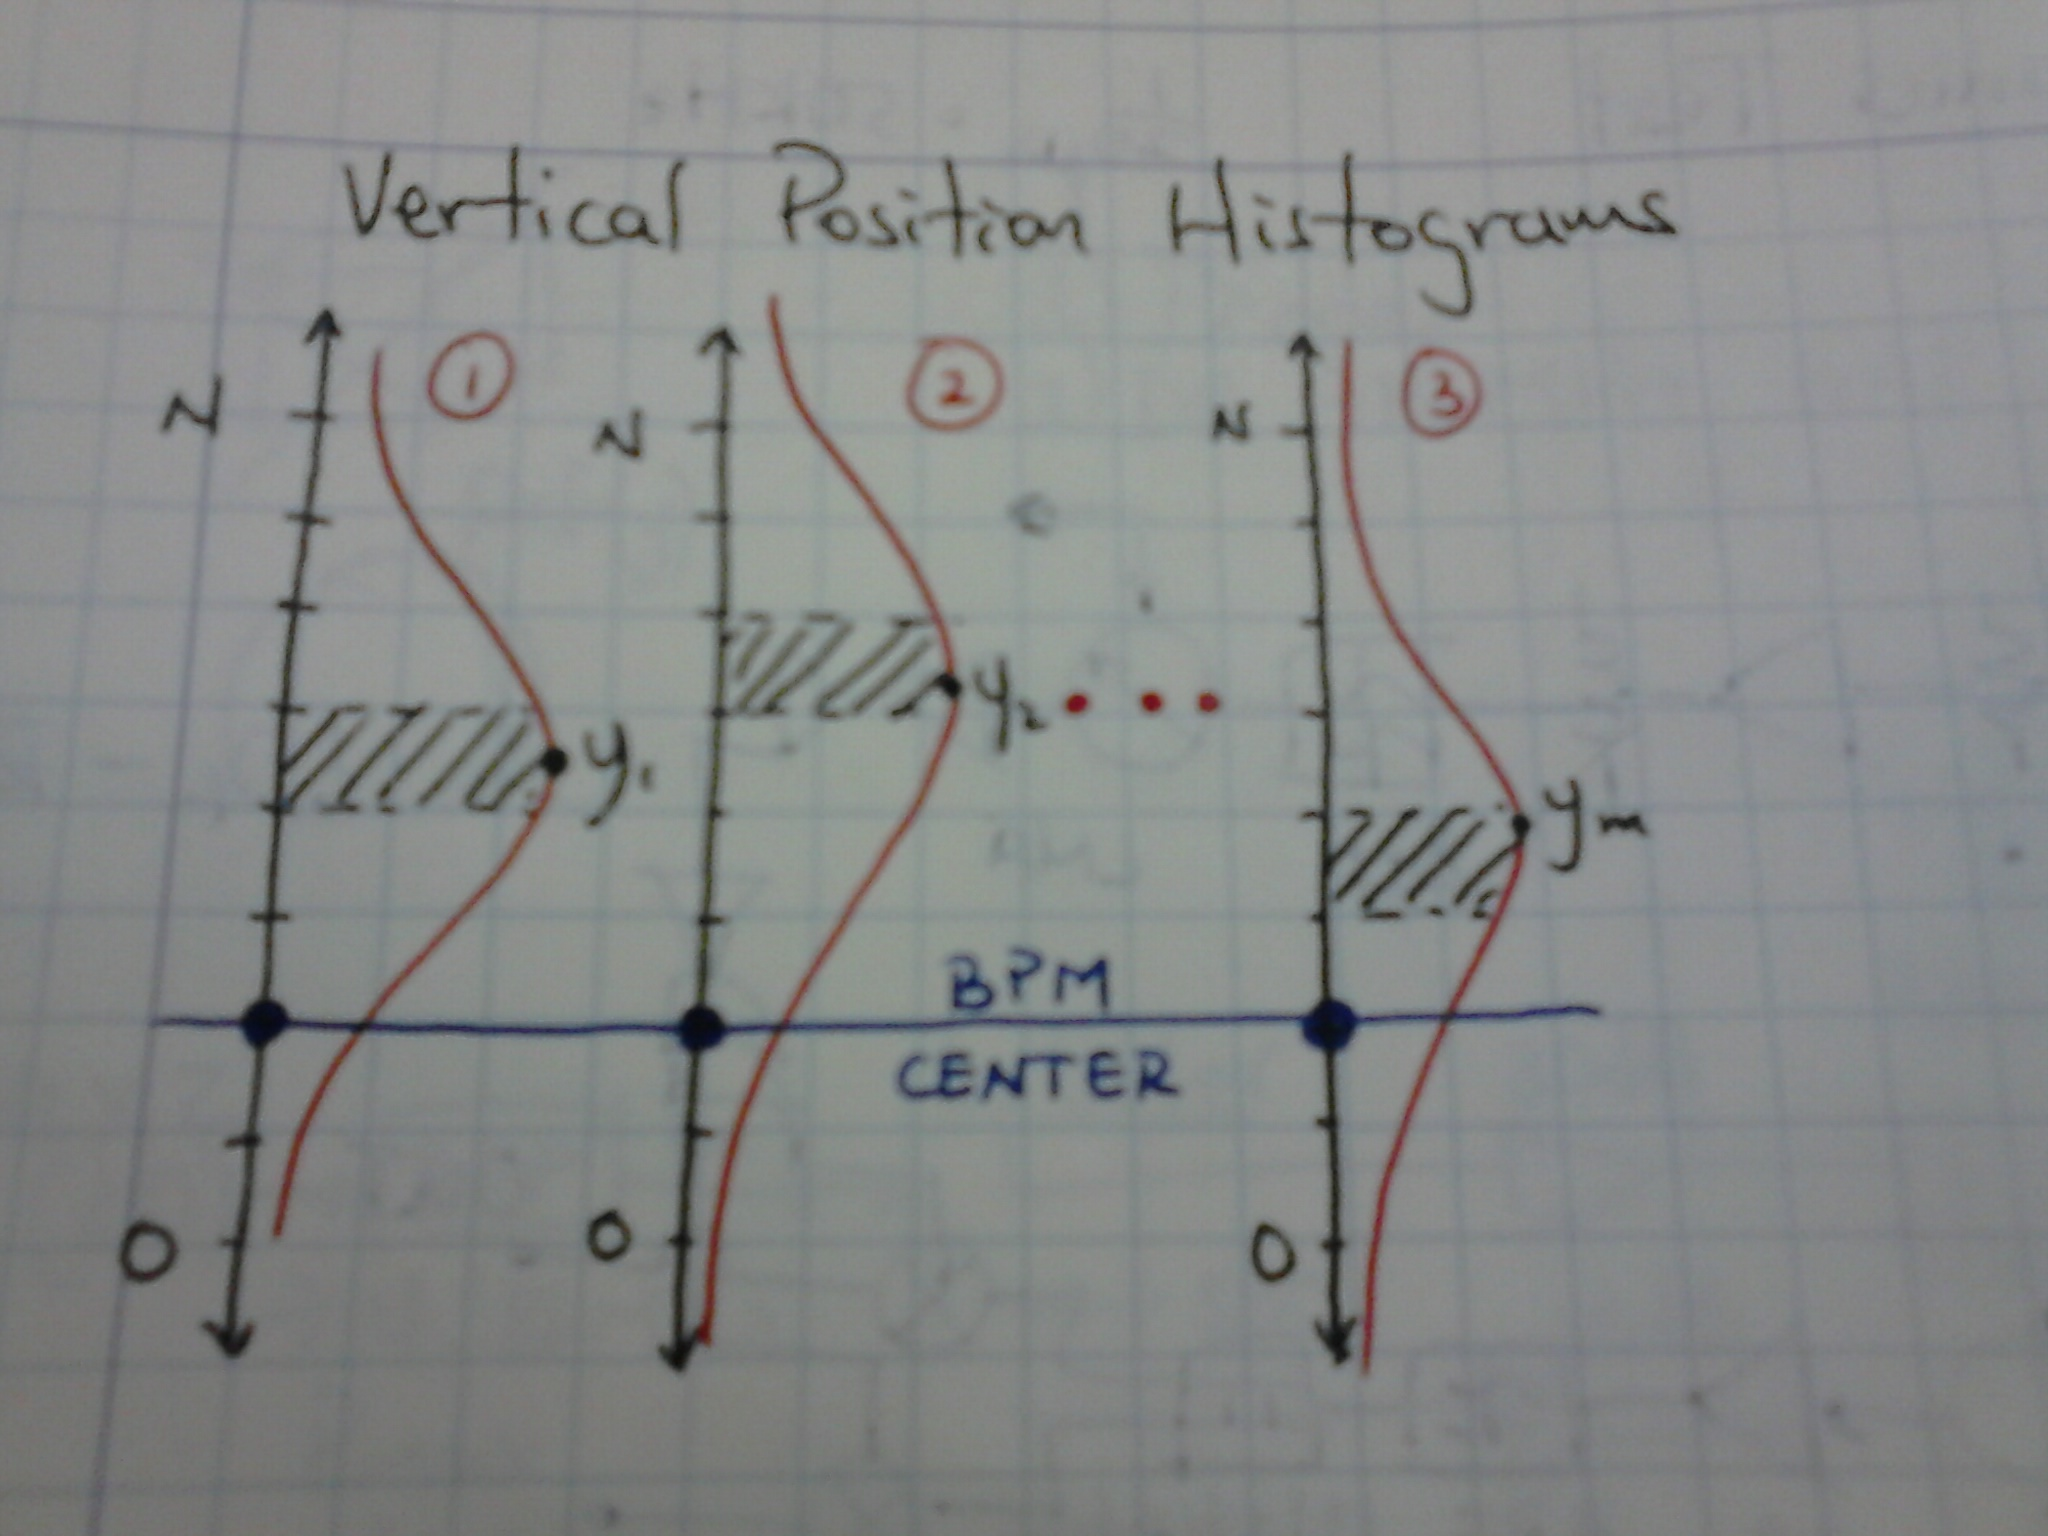
\includegraphics[angle=0,scale=0.1]{DSC_0026.jpg}\caption{Beam distr.}\label{beamdist}
 \end{center}
\end{figure}
Each vertical measurement $y_k$ is displaced from BPM center in an amount determined by a vertical offset $y_0$ with respect to cavity center and a random number proportional to beamsize ($y_{jk}=p\sigma_y$, and $p$ between 10 to 20\%, jitter). Therefore, from a sample $Y$ of $m$ bunches measured, $y_0=\langle Y\rangle$ and $\sigma_j^2=\langle Y^2\rangle-\langle Y\rangle^2$. In the case of one bunch, $y_{jk}=y_k-y_0$. Jitter will also be present in horizontal position and angles. For the moment, only discretisation level will be the only error source contributing to each $y_k$.\par
The objective is to measure $\boldsymbol{y_j}$ with \textbf{1nm} or $\boldsymbol{10^{-4}}$ relative precision for a bunch ($k$=1).\par
The preceeding statament means that the scale division used to measure $y$ should comply with\par
\begin{equation}
  \frac{y_j}{N}\leq1\text{nm, or, }\frac{1}{N}\leq10^{-4}
\end{equation}
In order to satisfy both, $N>10^{4}$. It also sets two ranges for the jitter measurement:
\begin{itemize}
 \item $y_j<10\mu$m, where resolution is below 1nm.
 \item $y_j\geq10\mu$m, where resolution is $10^{-4}$ maximum.
\end{itemize}
The maximum number counts used to measure jitter will always be below 10000. If we consider jitter conviniently centered, then it will be 5000 counts below $N/2$ and 5000 counts above $N/2$. The allowed offset under this circumstances, will be from 5000 counts to $N-5000$ counts. In total we have substracted 10000 counts from the total range, and the maximum offset will be $N-10000$ counts.\par
The number of counts $N$ comes from the binary $2^b$ discretisation scale where $b$ is the number of bits. As oscilloscopes are only 8 bits, the max. resolution will be around $10^{-2}$ ($2^8$). For a system with 14 bits, $N=16384$,  6384 counts are free for tolerances to different effects including offset. Any offset below $6.384\mu$m will will allow 1nm precision. Above this size, only $10^{-4}$ might be reached.\par
Table \ref{toletab} shows the different level of tolerances corresponding to different precision levels for 1nm resolution and 14 bits discretisation.\par
\begin{table}[hbt]
\begin{center}
 \begin{tabular}{|c|c|c|}\hline
 Precision & Total OFFSET SIGNAL ($\mu$m) & Centered ($\mu$m)\\\hline
 $10^{-2}$ &16.824&$\pm$8.142 \\\hline
 $10^{-3}$ &15.384&$\pm$7.692\\\hline
 $10^{-4}$ &6.384&$\pm$3.192\\\hline
 \end{tabular}
 \caption{Tolerances and precision.}\label{toletab}
 \end{center}
\end{table}
Consider now the signal $S$ as the sum of the two outputs from the cavity (which are ideally 180\degre separated) as seen in figure \ref{Ssignal},\par
\begin{figure}[htb]
 \begin{center}
  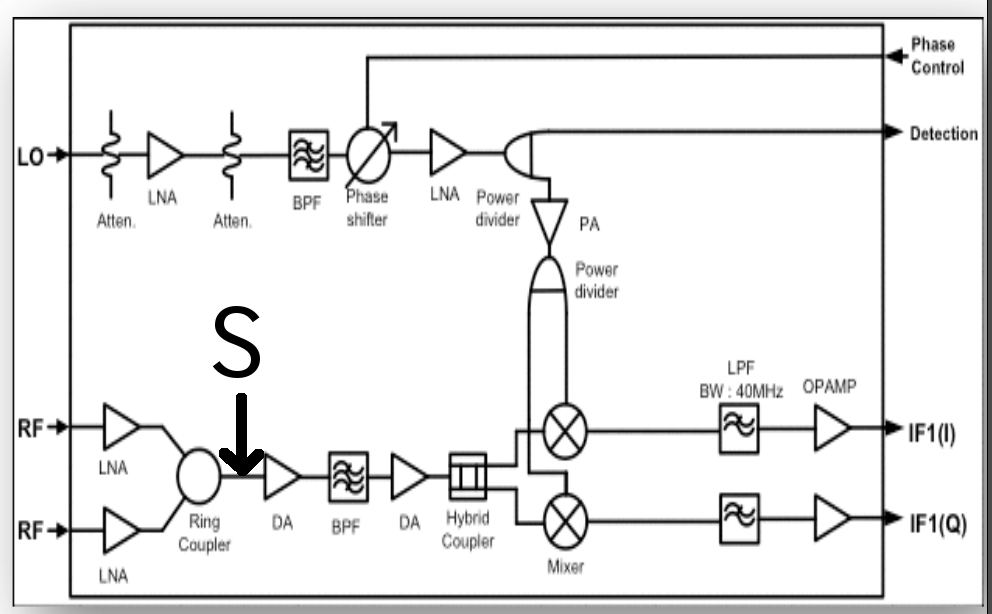
\includegraphics[angle=0,scale=0.4]{electr2.jpg}\caption{Signal S.}\label{Ssignal}
 \end{center}
\end{figure}
Signal $S$ for the vertical outputs of one BPM and one bunch is composed of:
\begin{equation}
S = y+is_p\theta_p+s_{xy}(x+is_y\theta_y)+x\theta_r
\end{equation}
where $i$ is the imaginary number indicating a 90 degrees phase difference (angle signals have 90 phase difference with respect to position signals from cavity). $s_p$ is the sensitivity to pitch angle, $s_{xy}$ is the inverse of X-Y isolation, $s_y$ is the yaw angle sensitivity. $x,y,\theta_p,\theta_r,\theta_y$, are horizontal position, vertical position, pitch, roll and yaw angles BPM with respect to beam.\par
Signal $S$ can be separated in real and imaginary parts:
\begin{equation}
S = (y+s_{xy}x+x\theta_r)+i(s_p\theta_p+s_{xy}s_y\theta_y)
\end{equation}
This signals are rotatated by an arbitrary angle $\phi$ to obtain the $I'$ and $Q'$ at the phase shifter block.
\begin{align*}
S &= \underbrace{(y+s_{xy}x+x\theta_r)(\cos\phi+i\sin\phi)}+\underbrace{i(s_p\theta_p+s_{xy}s_y\theta_y)(\cos\phi+i\sin\phi)}\\
  &= I' + Q' 
\end{align*}
In the case of perfect IQ rotation ($\phi=0$), all imaginary (angle and others) component is removed from real (position) component in the $S$ signal. However, in practice this rotation could be achieved to precision set by $\Delta\phi$, then, to first order
\begin{equation}
 S = [(y+s_{xy}x+x\theta_r)+\Delta\phi(s_p\theta_p+s_{xy}s_y\theta_y)]+i[\Delta\phi(y+s_{xy}x+x\theta_r)+(s_p\theta_p+s_{xy}s_y\theta_y)]
\end{equation}
where all term have been considered positive as they represent halved tolerances (positive-negative, $\pm$, errors). At this point will be only interested in the real part as it contains most of the vertical position signal.
\begin{equation}
 \Re[S]=S_y = (y+s_{xy}x+x\theta_r)+\Delta\phi(s_p\theta_p+s_{xy}s_y\theta_y)
\end{equation}
The last equation shows the contribution to vertical signal from the relative position BPM to beam.\par
Mean value of $S_y$ signal over $m$ bunches sample will be equal to
\begin{equation}
 \langle S_y\rangle = [y_0+s_{xy}(x_0+\eta\delta)+(x_0+\eta\delta)\theta_{r0}]+\Delta\phi[s_p\theta_{p0}+s_{xy}s_y(\theta_{y0}+\eta'\delta)]
\end{equation}
where all 0-index correspond to misaligment, $\eta$ and $\eta'$ are the dispersion and dispersion angle optic parameters, $\delta=10^{-3}$ is the energy spread, and no beam rotation is considered. $\langle S_y\rangle$ contribution to signal should be then below the values listed in Table \ref{toletab}.\par
Isolation X-Y (1/$s_{xy}$) was measured to be under 50dB (Pin/Pout$<10^{-5}$), sensitivity to pitch ($s_p$) was measured to be $3.2\mu$m/mrad, and sensitivity to yaw ($s_y$) is 2.9$\mu$m/mrad estimated in similar way to $s_p$. Precision on phase rotation ($\Delta\phi$) is still to be determined.\par

From this point, it will be assumed that mechanical positions could be measured within an absolute error shown in Table \ref{mechprec}.\par
\begin{table}[htb]
\begin{center}
 \begin{tabular}{|c|c|}\hline
  Axis & Mechanical Precision ($\mu$m)\\\hline
  Vertical & 1\\
  Horizontal & 5\\
  Longitudinal & 5 \\\hline
 \end{tabular}\caption{Position mechanical precision}\label{mechprec}
 \end{center}
\end{table}
Assuming that angles can be estimated from two coplanar points in the BPM, then, minimum resolvable angle might be within the values shown in Table \ref{angleprec}. Figure \ref{PAcontrol} shows the approximate location of angle control points.\par
\begin{table}[htb]
 \begin{center}
  \begin{tabular}{|c|c|c|}\hline
  Angle (Symbol) & Estimated min. resolvable value (mrad) & Distance between points (mm)\\\hline
   Pitch ($\theta_p$)&0.042&120\\
   Yaw ($\theta_y$)&0.042&120\\
   Roll ($\theta_r$)&0.033&30\\\hline
  \end{tabular}\caption{Angle mechanical precision}\label{angleprec}
 \end{center}
\end{table}
\begin{figure}[htb]
 \begin{center}
  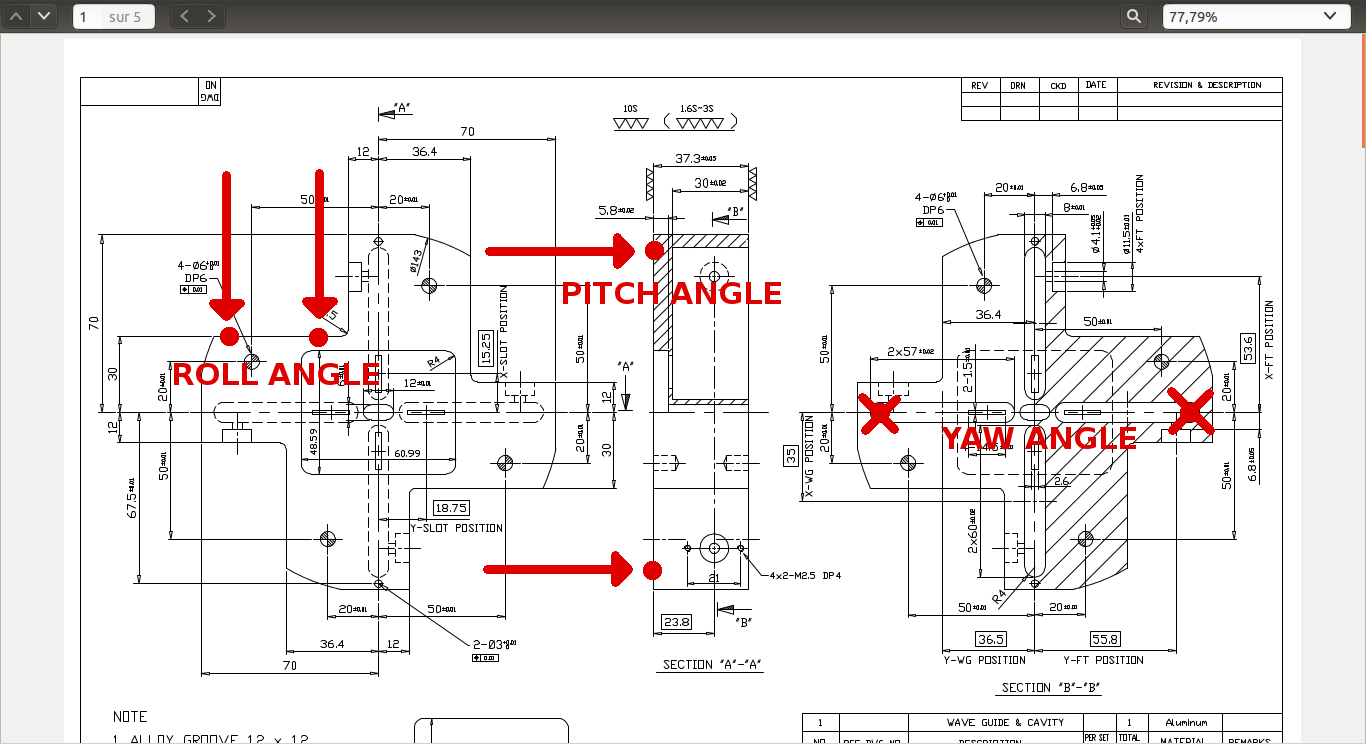
\includegraphics[angle=0,scale=0.4]{angles.jpg}\caption{Points of position and angle control.}\label{PAcontrol}
 \end{center}
\end{figure}
Using the nominal optics 1BX1BY, there are two relevant cases:
\begin{itemize}
 \item Largest beam size: it is at IPBPMA, having 57.657$\mu$m of vertical beam size. Jitter will be around 11.531$\mu$m (20\%)and 5.766$\mu$m (10\%). Both cases are close or inside of the 1nm resolution.
 \item Beam waist at the IP: in this case vertical beams size is 37$\sim$54nm, and beam jitter will be around 4$\sim$10nm. It is clearly inside the 1nm resolution case, however, SNR (Signal to Noise Ratio) must be considered in order to be able to separate jitter from other sources.
\end{itemize}
\subsection{Beam waist at IP and readings in IPBPMA}
The first case is the simplest one, as resolution is enough to get jitter measurement and a minimum of 6$\mu$m tolerance for all effects. $\eta=20.99\times10^{3}\mu$m, $\eta'=139.6$mrad. Tolerance will be deliverately distributed in the way shown in Table \ref{jsources}.
\begin{table}[htb]
 \begin{center}
  \begin{tabular}{|c|c|c|c|}\hline
  Final contribution to vertical signal ($\mu$m) & Symbol & Adition &Considered sources\\\hline
   2 & $y_0$ & 2$\mu$m & $y_0$\\
   1 & $x$ & 300$\mu$m & $x_j$(8)+$\eta\delta$(30)+$x_0$(5)\\
   1 & ($\theta_y$)&3mrad&$x'_j$(0.052)+$\eta\delta$(0.1)+$x_0$(5)\\
   Pitch ($\theta_p$)&&0.042&120\\
   Roll ($\theta_r$)&&0.033&30\\\hline
  \end{tabular}\caption{Tolerances}\label{jsources}
 \end{center}
\end{table}
